\documentclass[12pt,a4paper]{article}

% Required packages
\usepackage[utf8]{inputenc}
\usepackage[T1]{fontenc}
\usepackage{geometry}
\usepackage{graphicx}
\usepackage{booktabs}
\usepackage{hyperref}
\usepackage{enumitem}
\usepackage{tikz}
\usetikzlibrary{shapes.geometric, arrows, positioning}

% Page geometry
\geometry{top=1in, bottom=1in, left=1in, right=1in}

% Flowchart styles
\tikzstyle{startstop} = [rectangle, rounded corners, minimum width=3cm, minimum height=1cm,text centered, draw=black, fill=white]
\tikzstyle{process} = [rectangle, minimum width=3cm, minimum height=1cm, text centered, draw=black, fill=white]
\tikzstyle{decision} = [diamond, minimum width=3cm, minimum height=1cm, text centered, draw=black, fill=white]
\tikzstyle{arrow} = [thick,->,>=stealth]

\begin{document}

% Title Page
\begin{titlepage}
    \centering
    \scshape
    \vspace*{1cm}
    {\huge\bfseries Software Requirements Specification\par}
    \vspace{0.5cm}
    {\Large For Smart Gate System\par}
    \vspace{1.5cm}
    {\large Standard: IEEE 830-1998 (Agile-Integrated)\par}
    \vspace{2cm}
    
    \begin{table}[h]
        \centering
        \begin{tabular}{ll}
            \textbf{Version:} & 1.1 \\
            \textbf{Methodology:} & Agile Scrum \\
            \textbf{Lead Developer:} & Pratibha \\
            \textbf{Date:} & March 11, 2026
        \end{tabular}
    \end{table}

    \vspace{2cm}
    \textbf{Project Status:}\\
    Professional Phase 2 Deployment
    
    \vfill
    {\large Semester Project: Software Engineering\par}
    {\large \today\par}
\end{titlepage}

\tableofcontents
\newpage

\section{Introduction}
\subsection{Purpose}
This document specifies the requirements for the Smart Gate System (SGS). It serves as the primary technical baseline for development and academic evaluation.

\subsection{Project Scope}
The SGS aims to replace manual security logs with a digital, verifiable system.
\begin{itemize}
    \item \textbf{Phase 1}: Minimum Viable Product (MVP) with local registration and OTP.
    \item \textbf{Phase 2}: Enterprise features including Firebase Auth and Testmail.app QR delivery.
\end{itemize}

\section{System Architecture \& Workflow}

\subsection{Visitor Entry Flowchart}
Below is the logical flow for a visitor entering the premises using the Testmail.app integration:

\begin{center}
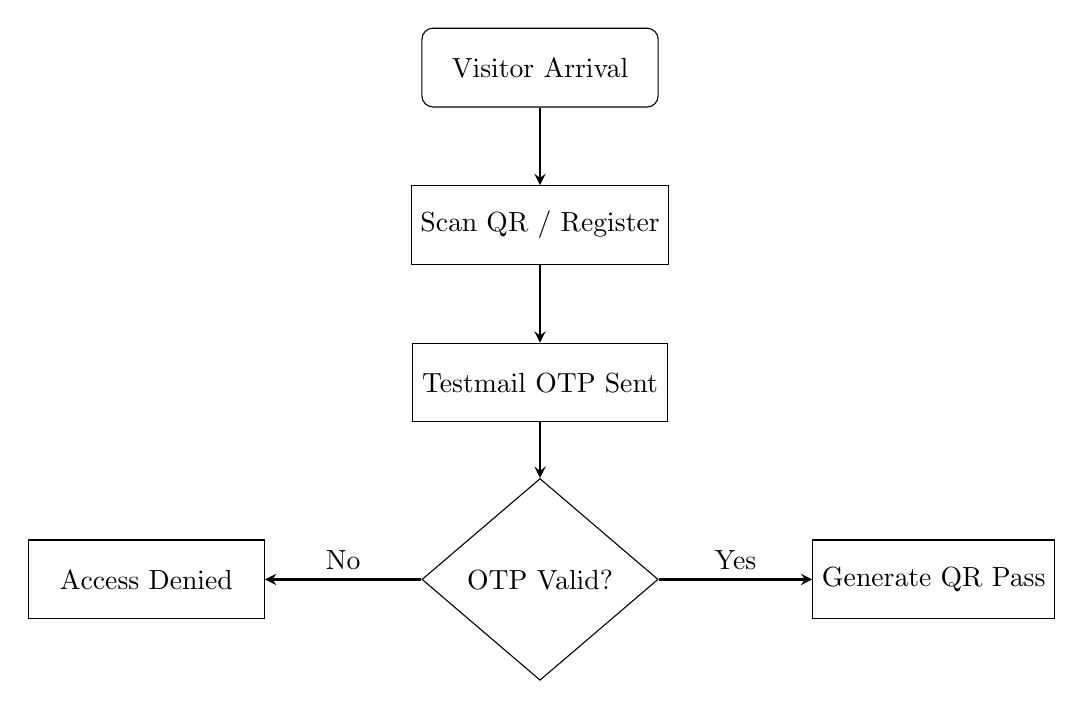
\begin{tikzpicture}[node distance=2cm]
    \node (start) [startstop] {Visitor Arrival};
    \node (reg) [process, below of=start] {Scan QR / Register};
    \node (otp) [process, below of=reg] {Testmail OTP Sent};
    \node (verify) [decision, below of=otp, yshift=-0.5cm] {OTP Valid?};
    \node (grant) [process, right of=verify, xshift=3cm] {Generate QR Pass};
    \node (deny) [process, left of=verify, xshift=-3cm] {Access Denied};
    
    \draw [arrow] (start) -- (reg);
    \draw [arrow] (reg) -- (otp);
    \draw [arrow] (otp) -- (verify);
    \draw [arrow] (verify) -- node[anchor=south] {Yes} (grant);
    \draw [arrow] (verify) -- node[anchor=south] {No} (deny);
\end{tikzpicture}
\end{center}

\section{Specific Requirements}
\subsection{Functional Requirements}
\begin{enumerate}[label=FR.\arabic*]
    \item \textbf{Registration}: System shall allow registration via mobile link.
    \item \textbf{Verification}: System shall verify visitors via 6-digit OTP sent through Testmail.app.
    \item \textbf{Authentication}: System shall use Firebase for Guard and Admin secure login.
    \item \textbf{Blacklist}: System shall cross-reference numbers against a security blacklist.
\end{enumerate}

\subsection{Non-Functional Requirements}
\begin{itemize}
    \item \textbf{Security}: Firebase and JWT-based session management.
    \item \textbf{Performance}: API responses under 500ms.
\end{itemize}

\section{Timeline \& Sprints}
\begin{table}[h!]
    \centering
    \begin{tabular}{|l|l|}
        \hline
        \textbf{Sprint} & \textbf{Focus} \\ \hline
        Sprint 0-1 & Setup \& Core API (Pratibha) \\ \hline
        Sprint 2 & OTP Logic \& Local Auth (Pratibha) \\ \hline
        Sprint 3-4 & Firebase \& Testmail.app (Pratibha) \\ \hline
    \end{tabular}
    \caption{Agile Development Schedule}
\end{table}

\end{document}
